\documentclass[twoside]{article}

\usepackage[margin=4cm]{geometry}
\usepackage{calligra}
\usepackage[colorlinks, linkcolor=azulsema!60!black]{hyperref}
\usepackage{wrapfig}
\usepackage{multicol}
\usepackage{subfigure}
\usepackage{eurosym}
%\usepackage[latin1]{inputenc}
\usepackage[T1]{fontenc}
\usepackage[spanish]{babel}
\usepackage{colortbl}
\usepackage{float}

\usepackage{tikz}

\begin{document}

\subsection{Control and Related Fields}
\begin{center}
\textbf{Sevilla, Marzo 27-29, 2023 (España)}\\[.5em]
\url{ http://departamento.us.es/edan/CRF23/}\\[.5em]

\includegraphics[width=0.3\linewidth]{images/us}
\quad 

\includegraphics[width=0.25\linewidth]{images/imus2}
\quad 

\includegraphics[width=0.2\linewidth]{images/logoEDAN} 
\end{center}
 
 
 
 \bigskip
 
En las fechas del 27 al 29 de marzo de 2023 en el  Instituto de Matemáticas de la Universidad de Sevilla se ha celebrado el  Workshop \textbf{Control and Related Fields}. La temática principal del workshop se ha centrado en la teoría del control y campos afines: problemas de identificación y técnica de dispersión inversa, problemas de control óptimo, así como problemas de estabilización en ingeniería y métodos numéricos para problemas de control y problemas inversos.

Este evento ha reunido a investigadores internacionales (jóvenes y senior) del campo de la teoría de control. El objetivo de este evento ha sido ofrecer una visión amplia de este campo apasionante y poner de manifiesto su rápida evolución, así como facilitar el intercambio de ideas sobre los avances recientes en sus diversos aspectos.

Además, de las conferencias plenarias con ponentes senior (charlas de 50 minutos) y junior (charlas de 25 minutos) ha tenido lugar una sesión de pósters. 

La lista de los conferenciantes invitados es la que sigue.



\subsubsection*{Conferenciantes invitados}
 
\begin{itemize}
\item J. Apraiz (Universidad del País Vasco, Spain)
\item A. Benabdallah (Aix-Marseille University, France)
\item A. Benaissa (Djillali Liabes University, Algeria)
\item I. Boussaada (Paris-Saclay University, France)
\item C. Castro (Universidad Politécnica de Madrid, Spain)
\item A. Doubova (Universidad de Sevilla, Spain)
\item E. Fernández-Cara (Universidad de Sevilla, Spain)
\item F. Macià (Universidad Politécnica de Madrid, Spain)
\item C. Pignotti (Università dell'Aquila, Italy)
\item L. Robbiano (Paris-Saclay University, France)
\item M. Sepúlveda (Universidad de Concepción, Chile)
\item F. Triki (Grenoble Alpes University, France)
\item Z. Abdallah (Lebanese University, Lebanon)
\item J.A. Bárcena-Petisco (Universidad del País Vasco, Spain)
\item M. Ben Said (University of Monastir, Tunisia)
\item D. A. de Souza (Universidad de Sevilla, Spain)
\item K. Le Balc'h (Sorbonne Université, France)
\item I. Marín-Gayte (Universidade de Lisboa, Portugal)
\item S. Marx (Nantes Université, France)
\item W. Zouhair (Cadi Ayyad University, Morocco)
\end{itemize}

\bigskip
\begin{figure}[h!]
\centering
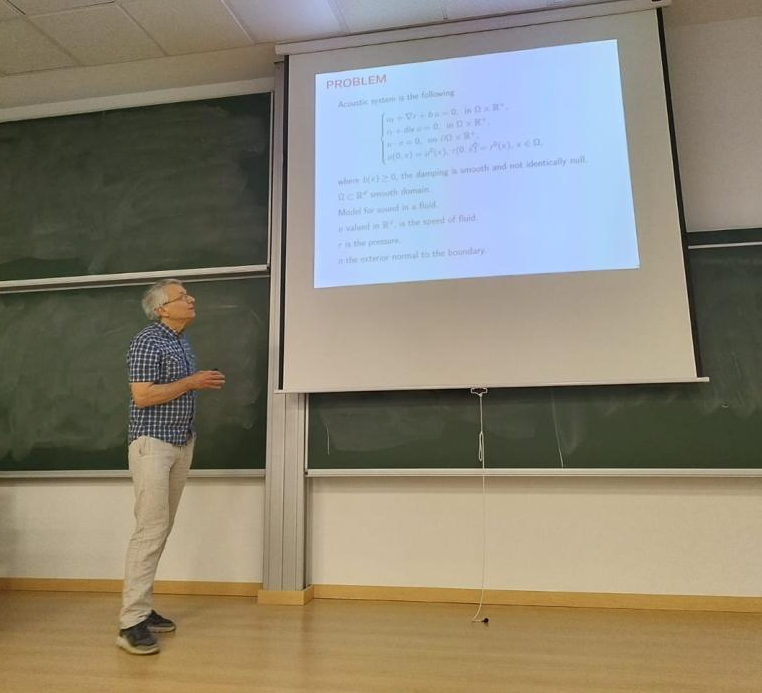
\includegraphics[width=0.7\linewidth]{images/Robbiano}
\caption{L. Robbiano (Paris-Saclay University, France).}
\end{figure}



\begin{figure}[h!]
\centering
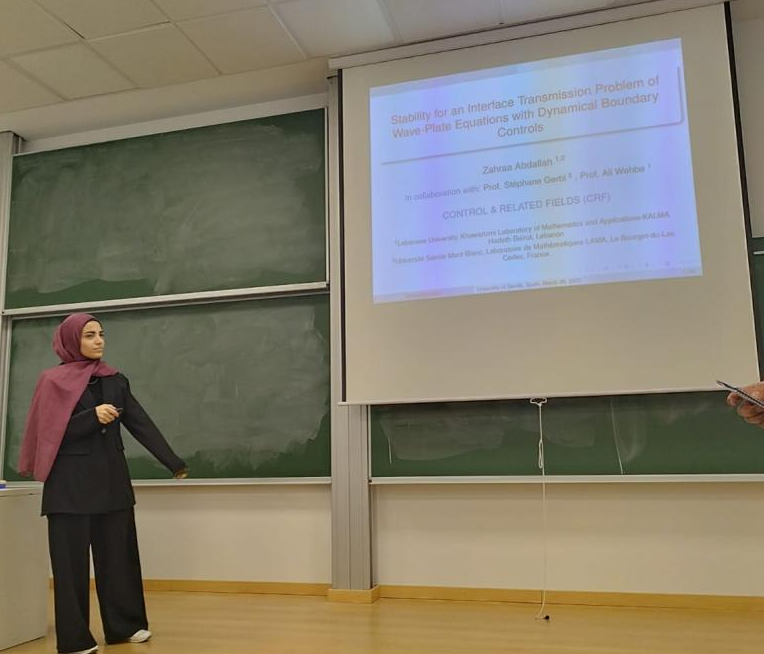
\includegraphics[width=0.7\linewidth]{images/ZahraaAbdallah}
\caption{Z. Abdallah (Lebanese University, Lebanon).}
\end{figure}


\begin{figure}[h!]
\centering
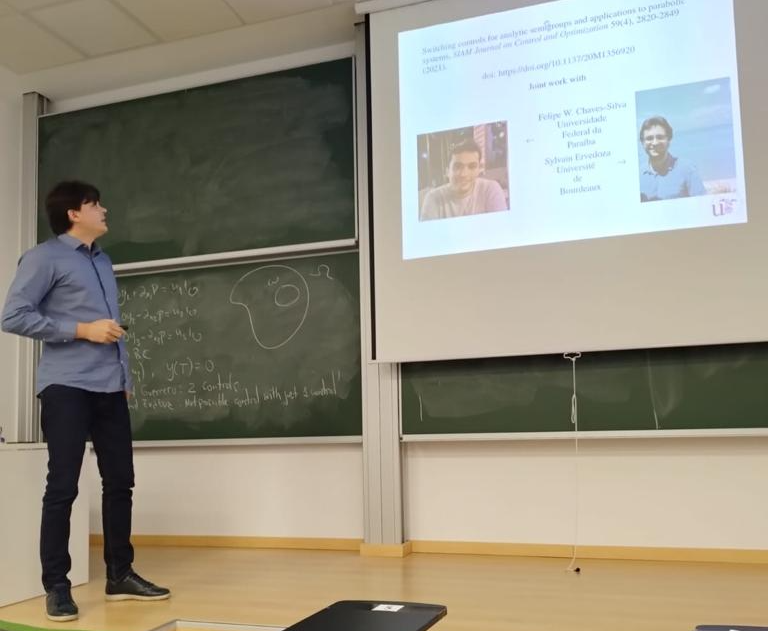
\includegraphics[width=0.7\linewidth]{images/Diego}
\caption{D. A. de Souza (Universidad de Sevilla, Spain).}
\end{figure}


\begin{figure}[h!]
\centering
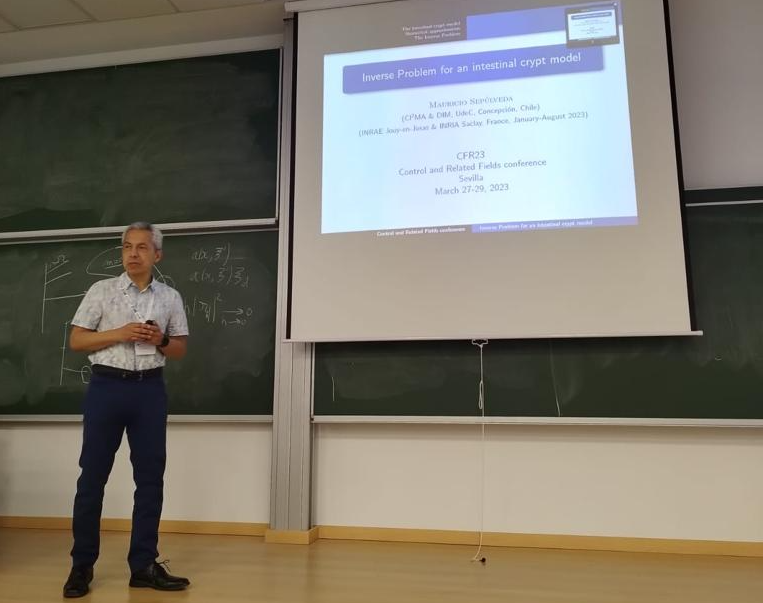
\includegraphics[width=0.7\linewidth]{images/MSepulveda}
\caption{M. Sepúlveda (Universidad de Concepción, Chile).}
\end{figure}


\begin{figure}[h!]
\centering
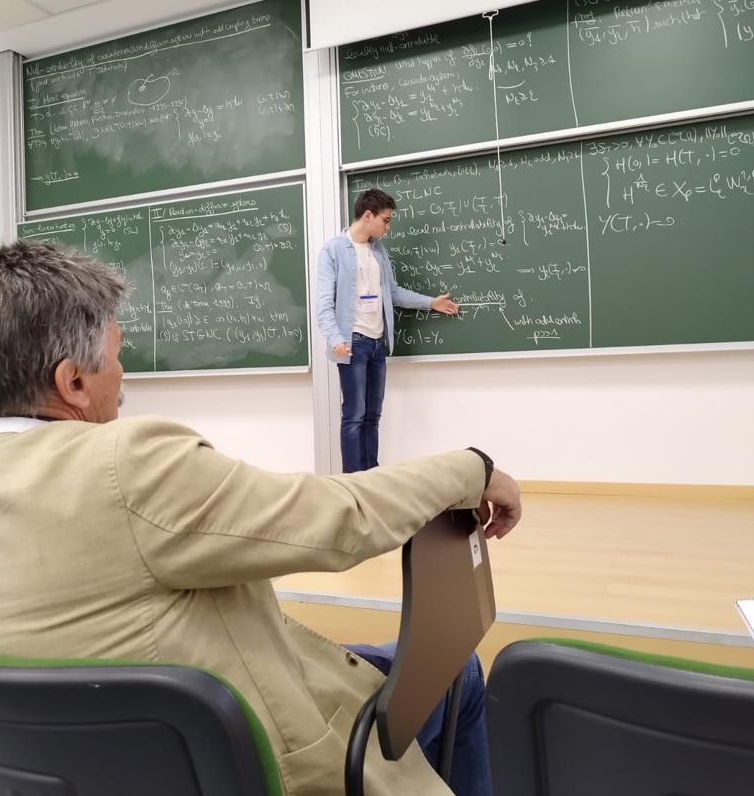
\includegraphics[width=0.7\linewidth]{images/Kevin}
\caption{K. Le Balc'h (Sorbonne Université, France).}
\end{figure}



\begin{figure}[h!]
\centering
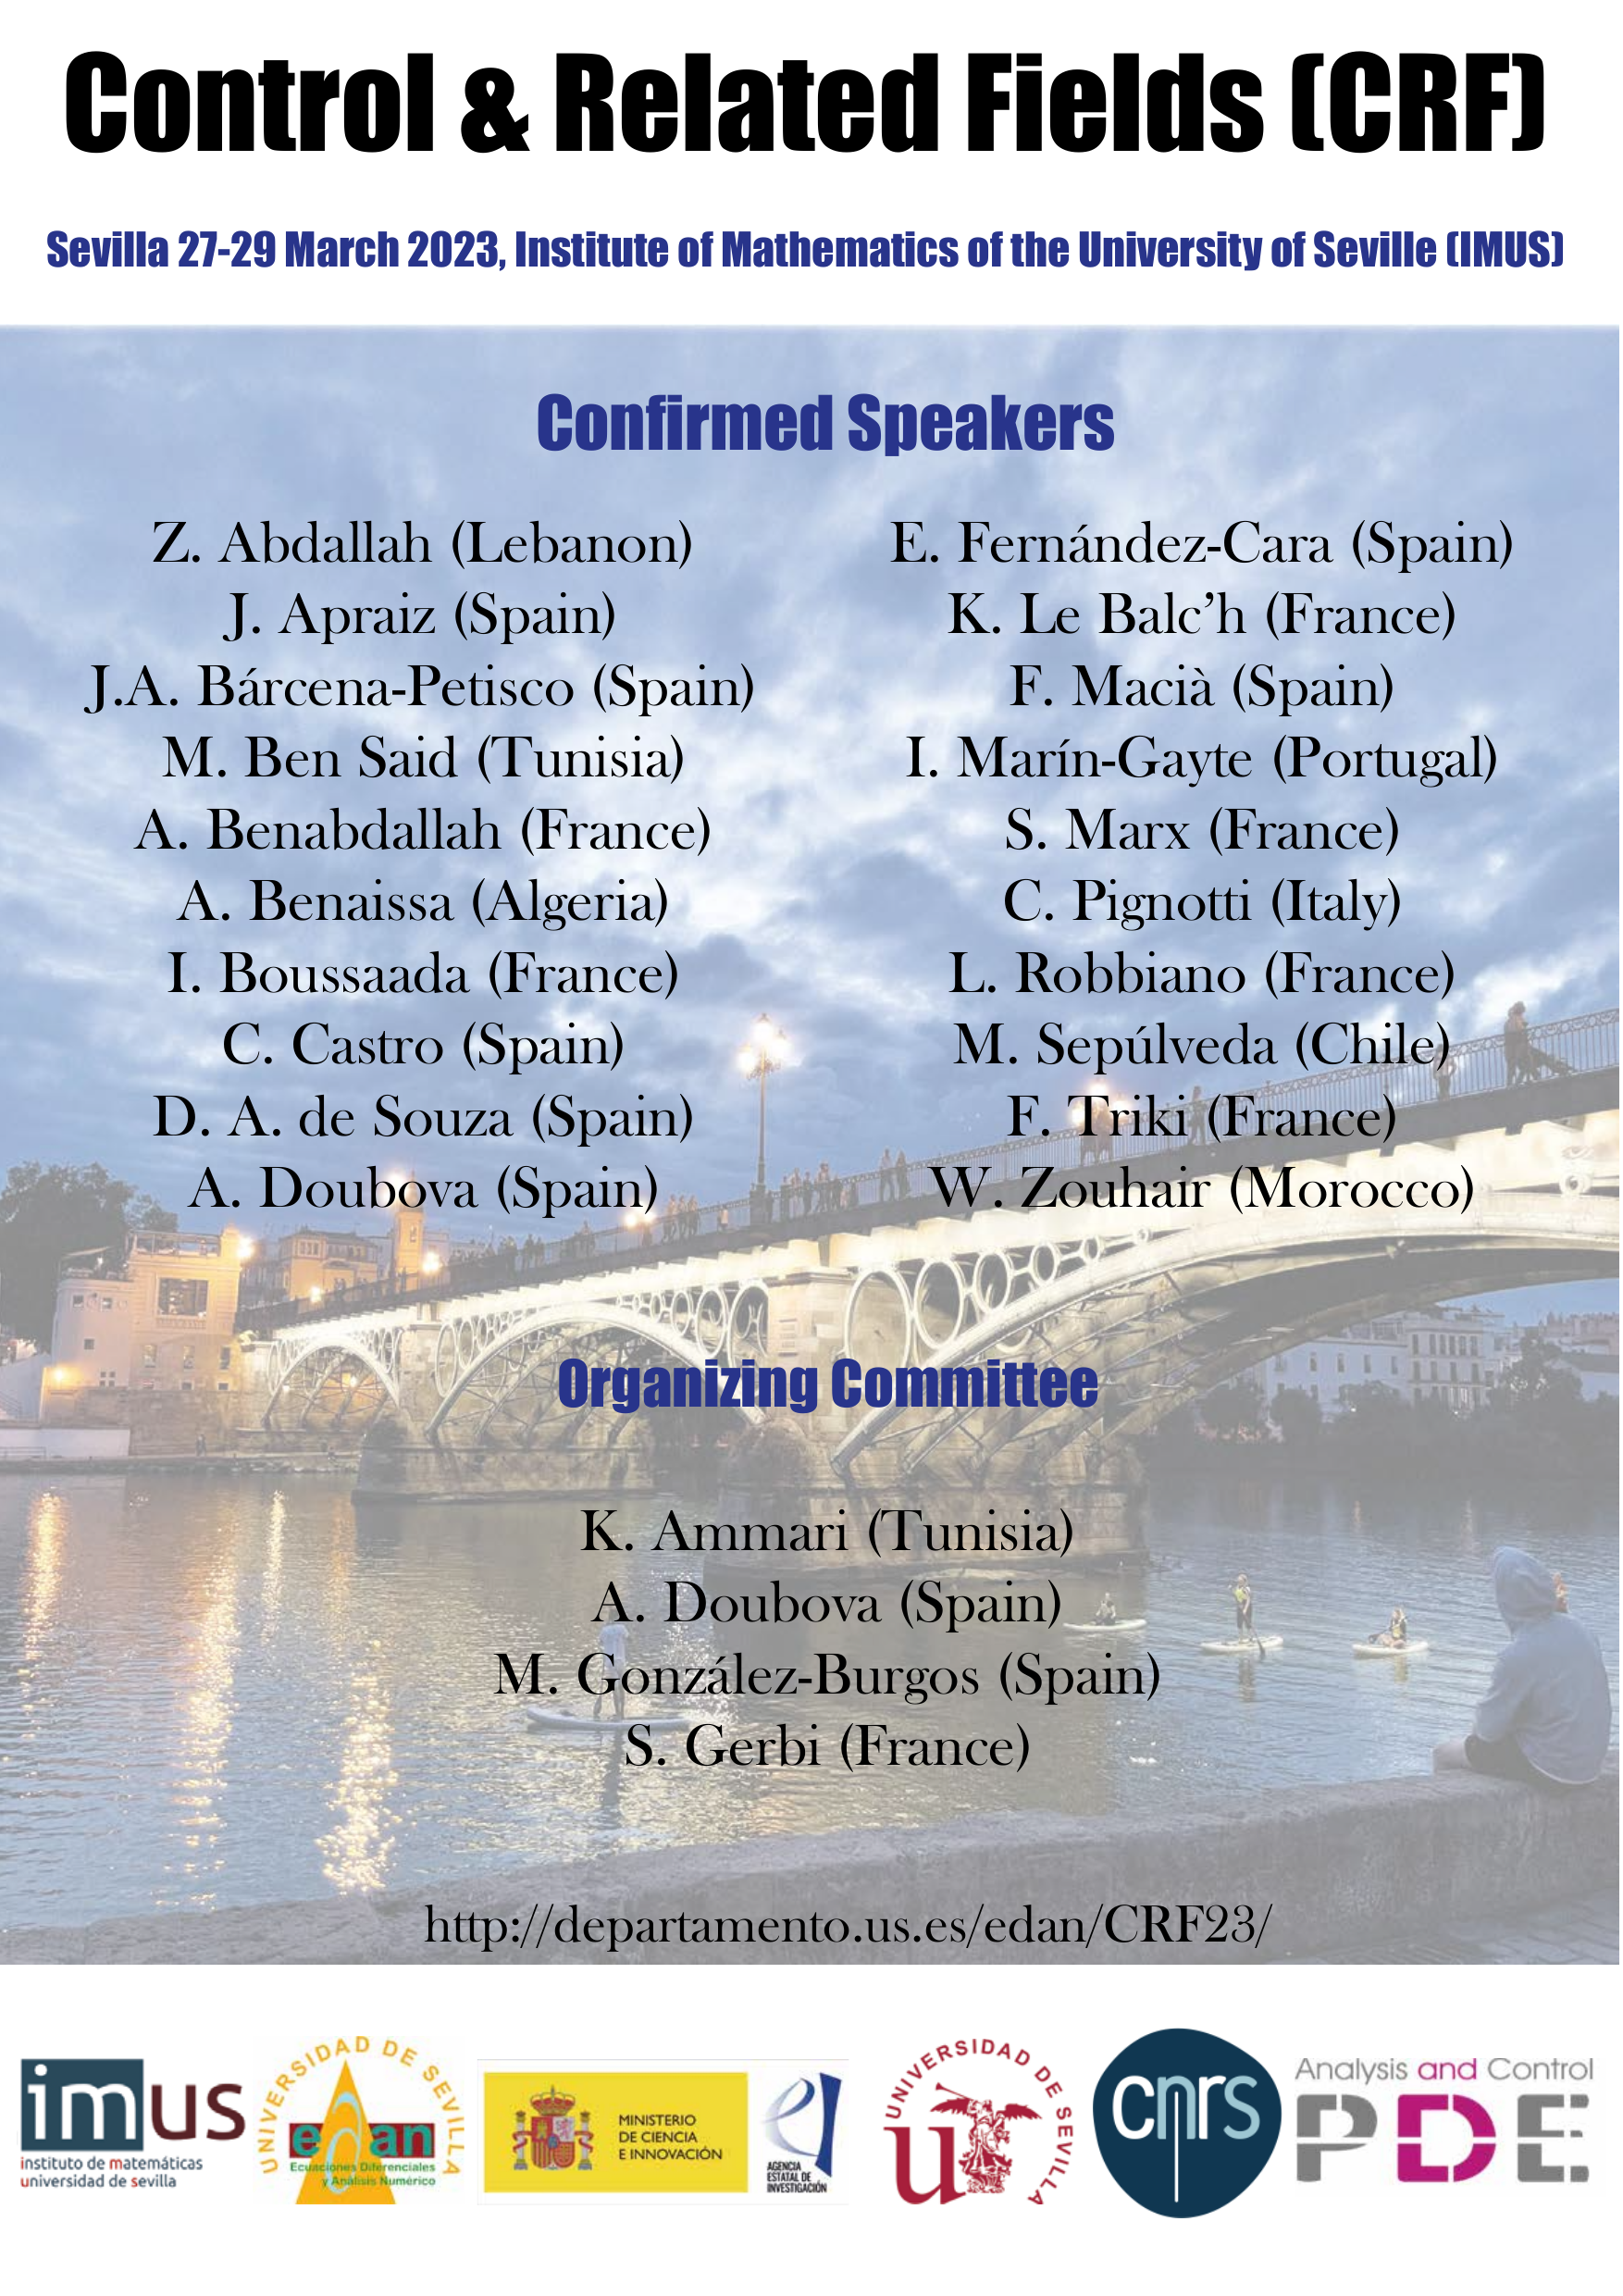
\includegraphics[width=0.99\linewidth]{images/posterCRF23}
\caption{Póster del congreso.}
\end{figure}

\end{document}
